\vspace{0.5cm}
\newline
\noindent\lecture{19}{16/12/2021}
\vspace{0.5cm}
\noindent Torniamo ora un attimo a descrivere i livelli energetici ricavati come autovalori dall'hamiltoniana di Jaynes-Cumming.
Supponiamo di disegnare in verticale, come linee orizzontali, i livelli energetici della cavità e, a fianco, i livelli energetici del qubit. Consideriamo anche un $\Delta < 0$. Per ora stiamo considerando come se non ci fosse alcuna interazione fra i due sistemi (ovvero $g=0$ o $\abs{ \Delta} \gg 0$). Ora aumentiamo l'interazione (diminuendo il \textit{detuning}): il livello eccitato del qubit si sposterà a energie inferiori, mentre quello della cavità si sposterà a energie superiori.
Nel caso $\Delta=0$ avremo i livelli eccitati che inizialmente sono uguali, ma verranno a crearsi due \textit{polarons states} dovuti all'ibridazione fra i due sistemi (uno inferiore rispetto agli originali viene detto $\ket{n-}$ e uno superiore $\ket{n+}$). La degenerazione iniziale, dunque, è rotta dall'interazione: tale fenomeno è spesso chiamato \textit{dynamic Stark splitting} (è causato dal campo elettrico della cavità e descritto dal termine dell'hamiltoniana $\propto \frac{g^2 n}{\Delta}$). Assieme ad esso si parla anche di \textit{Lamb shift}, per il termine non dipendente da $n$ ($\propto \frac{g^2}{\Delta}$). Si parla anche di \textit{Rabi splitting} poiché fondamentalmente provoca oscillazioni di Rabi (come abbiamo visto precedentemente).
\begin{figure}[H]
    \centering
    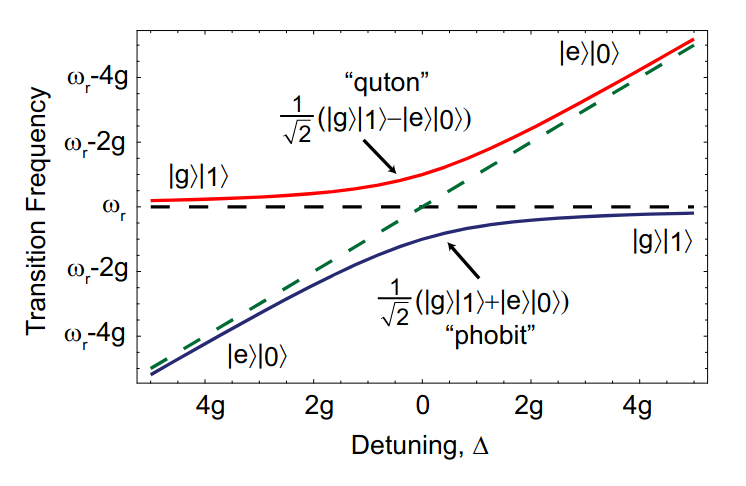
\includegraphics[width=0.6\textwidth]{images/avoided_crossing.png}
    \caption{A plot of the avoided crossing in the transition frequency between the ground state in the one excitation manifold. The dashed lines show the uncoupled resonator frequency, $\omega_r$ (black) and qubit frequency, $\omega_a$ (green). The solid red and blue lines show the energy for the $\ket{1+}$ and $\ket{1-}$ states as a function of detuning. At large detunings these energies and the associated eigenstates approach that of the uncoupled system. When $\Delta \rightarrow 0$ the photon and qubit become entangled forming “phobit” and “quton” states. \url{https://rsl.yale.edu/sites/default/files/files/RSL_Theses/SchusterThesis.pdf}}
\end{figure}
\noindent Le due frequenze, dunque, sono sottoposte ad \textit{avoided crossing} a causa dell'ibridizzazione degli stati. La minima differenza fra le due curve è proporzionale a $\propto g\sqrt{n+1}$ (perciò più l'accoppiamento è forte, più i livelli si allontanano).
Le oscillazioni di Rabi che vengono a crearsi, si stabiliscono fra uno stato $\ket{e, n}$ e lo stato $\ket{g, n+1}$ con una frequenza data dallo splitting fra i due livelli ibridati.
Consideriamo ora il limite dispersivo (il grafico a livelli che riportiamo è \textbf{diverso} da quello precedentemente descritto). Ogni stato si sposterà di $\abs{n\chi}$
\begin{figure}[H]
    \centering
    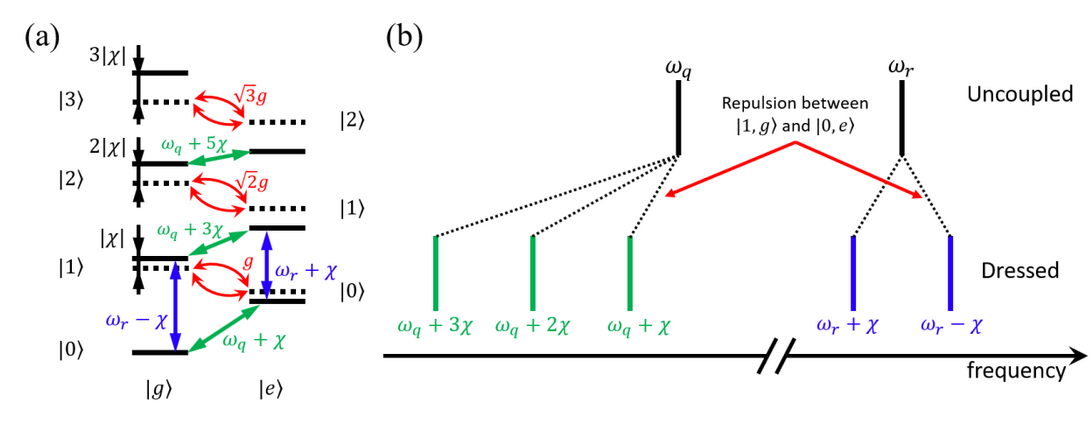
\includegraphics[width=\textwidth]{images/energy_split_disp_cqed.png}
    \caption{(a) Energy level diagram of a CQED system in the dispersive limit. Dotted black lines
denote the uncoupled bare basis and solid black lines denote the dressed basis. (b) Spectrum of
the uncoupled bare basis and the dressed basis. \url{https://drive.google.com/file/d/11HFMI_mos-a6GmhRrptYak8xe5h7oNzw/view}}
\end{figure}
\noindent Nella Figura (b) sono riportate in frequenza le possibili transizioni. Si vede che il qubit è sensibile al numero di fotoni presenti nella cavità: questo è problematico perché una certa fluttuazione in $n$ è inevitabile e sarà, dunque, una fonte di \textit{dephasing}.

\subsection{Oltre all'hamiltoniana di Jaynes-Cumming}
L'hamiltoniana complessiva dei due sistemi, in realtà, è data dalla somma dell'hamiltoniana di Jaynes-Cumming e due diversi termini:
\begin{equation*}
    H=H_{JC}+H_\gamma + H_k
\end{equation*}
I due termini aggiuntivi descrivono transizioni non considerate dall'hamiltoniana che abbiamo studiato fino ad ora. Ad esempio $H_k$ descrive la possibilità di fuga dei fotoni: questo termine è dunque legato a $k$, il rate di decadimento della cavità (si parla di accoppiamento della cavità col continuo o con l'ambiente). Possiamo scrivere:
\begin{equation*}
    k = \frac{\omega_c}{Q}
\end{equation*}
$Q$ è il fattore di qualità della cavità che descrive la larghezza della risonanza della cavità stessa e, dunque, la sua vita media. In particolare un alto $Q$ ci permette di distinguere al meglio le frequenze di transizione della cavità ed è perciò, preferibile. 
Invece $H_\gamma$ descrive l'accoppiamento fra qubit e modi di oscillazione diversi da quelli della cavità (ovvero descrive la probabilità che il qubit decada tramite fotoni alla frequenza "sbagliata"). Anche questo termine contribuisce, chiaramente, al valore del tempo di rilassamento.
$H_\gamma$ descrive, dunque, la larghezza delle frequenze della cavità (ed è un fattore largamente controllabile), mentre $H_k$ descrive la larghezza delle frequenze del qubit (ed è un fattore largamente intrinseco). Chiaramente i polarons avranno larghezza $(\gamma+k)/2$. 
\subsection{Charge qubit e CPW}

Nel caso di qubit superconduttivi, lo studio dell'accoppiamento cavità-qubit può essere affrontato diversamente.
Abbiamo detto che è possibile realizzare una cavità in modi diversi (ad esempio la cavità 3D). Siccome attualmente viene utilizzata maggiormente una cavità 2D (usando una CPW) ci concentreremo su questa realizzazione. Lo studio di tale cavità è piuttosto complicato, ma ci permette di definire in fase di progettazione tutte le sue caratteristiche: in particolare abbiamo che il fattore di merito $Q$ dipenderà dai valori capacitivi agli estremi della CPW e a seconda dei collegamenti fra linea di trasmissione e bulk. In generale si scrive:
\begin{equation*}
    \frac{1}{Q}= \frac{1}{Q_{int}}+ \frac{1}{Q_{ext}}
\end{equation*}
Dove $Q_{int}$ è il fattore di merito ottenuto considerando solo la CPW in sé e $Q_{ext}$ considera l'accoppiamento con l'esterno della CPW (ovvero le due capacità agli estremi).
Questa è una visione classica del sistema, chiaramente le formule subiranno alcuni cambiamenti con la quantizzazione del campo. In ogni caso rimangono i fattori di merito collegati al decadimento della cavità (ad esempio $Q_{ext}$ contiene informazioni sulla probabilità di un fotone interno di accoppiarsi con l'esterno).
Diamo qualche dimensione alla CPW: la linea di trasmissione interna sarà lunga all'incirca $1cm$ (e separata dal resto in modo da disaccoppiare la cavità), mentre lo spazio di dielettrico fra essa e i GND sarà generalmente nell'ordine di $10\mu m$. Un qubit (di circa $1\mu m$) può essere posizionato in posizione corrispondente al centro della cavità (dove la prima onda stazionaria raggiunge il suo massimo).
\begin{figure}[H]
    \centering
    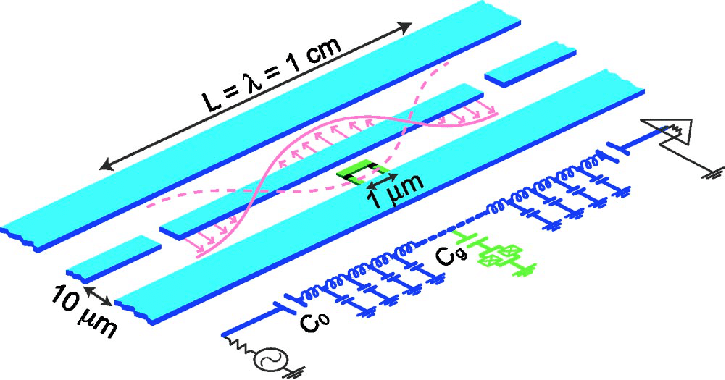
\includegraphics[width=0.5\textwidth]{images/cpw_cavity.png}
    \caption{\url{https://www.researchgate.net/publication/279263572_Coupling_quantum_dot_circuits_to_microwave_cavities}}
\end{figure}
\noindent La cavità, raffreddata abbastanza, si comporta come un oscillatore armonico con hamiltoniana:
\begin{equation*}
    \hat H= \hbar \omega_c \left( \hat a^\dagger \hat a + \frac{1}{2}\right)
\end{equation*}
Studiamo ora come avviene l'accoppiamento fra un qubit di carica (ne considero uno a doppia giunzione in modo da poter controllarne la frequenza caratteristica tramite una variazione dell'energia Josephson) e una cavità. 
L'hamiltoniana che abbiamo ricavato per questo qubit è:
\begin{equation*}
    \hat H= E_C ( \hat n - n_g)^2 -E_J \cos \delta
\end{equation*}
E non dobbiamo dimenticarci che l'operatore numero $\hat n = \hat a^\dagger \hat a$ veniva dal formalismo della seconda quantizzazione dopo aver reso discreti gli operatori (canonici) $\hat Q$ e $\hat \Phi$.
Possiamo anche identificare due diversi tipi di tensione: una "classica" che è quella utilizzata per controllare il numero di coppie di Cooper presenti sull'isola del qubit e una "quantistica" e quantizzata data da: $\hat V = \hat Q / C$.
Avevamo definito $n_g = \frac{C_g V_g}{2e}$ (capacità e tensione di gate). Ora sostituiamo a $V_g$ la tensione totale: $V_g \rightarrow \frac{\hat Q}{C}+V_{g}$. In questo modo arriviamo a ridefinire $n_g$:
\begin{equation*}
    \hat n_g = \frac{C_g (V_g + \hat V)}{2e}
\end{equation*}
Dunque la parte elettrostatica dell'hamiltoniana è scrivibile come (rimuovo i termini costanti):
\begin{equation*}
    \hat H = E_C (\hat n -  n_g)^2 - E_C C_g \frac{\hat V \hat n}{e}
\end{equation*}
Vale anche la relazione (con il parametro modulabile e compreso fra 0 e 1: $\beta=C_g/C_{TOT}$):
\begin{equation*}
    \frac{E_C C_G}{e} = \frac{2e}{C_{TOT}}C_g = 2 e \beta
\end{equation*}
Dunque posso scrivere il secondo termine dell'hamiltoniana elettrostatica come:
\begin{equation*}
    2e\beta V_0 (\hat a^\dagger + \hat a ) \hat n
\end{equation*}
Con $V_0=V_{\text{ZPF}}=\sqrt{\frac{\hbar \omega_c}{CL}}$. Questo è il termine che causa l'accoppiamento fra campo della cavità e qubit anche in assenza di fotoni. Nel caso $Q=10\,GHz$ e le dimensioni sopraindicate della cavità avremo $V_0 \sim 2\, \mu V$ (un valore non trascurabile) e un campo $E\sim 0.2\, \frac{V}{m}$ (circa 100 volte superiore al campo ottenibile nel caso di atomi reali).
Il termine $g$ di accoppiamento è:
\begin{equation*}
    g = \frac{eV_0\beta}{\hbar}
\end{equation*}
Benché abbiamo intuito da dove viene il termine di accoppiamento $g$, non abbiamo ancora trovato la corretta hamiltoniana di Jaynes-Cumming.
\subsubsection{Cooper Pair Box}
Analizziamo inizialmente il caso di una \textit{Cooper Pair Box}.
Ricordiamo che, per una CPB, abbiamo $E_C \gg E_J$ e l'hamiltoniana (ridotta a due livelli) si può scrivere come:
\begin{equation*}
    H = -\frac{E_C}{2}(1-2n_g)\sigma_z + \frac{E_J}{2}\sigma_x - 2 \hbar g (a^\dagger + a )\hat n+H_C
\end{equation*}
L'ultimo termine è quello su cui ancora dobbiamo lavorare (benché sappiamo che $\hat n \propto \sigma_z$).
Quando abbiamo studiato le CPB abbiamo detto che, per raggiungere la forma corretta dell'hamiltoniana per il sistema a due livelli, era necessario ruotare gli assi $x$-$z$ per un angolo $\theta=\arctan\left( \frac{E_J}{E_C(1-2n_g)}\right)$. Così facendo, i primi due termini dell'hamiltoniana appena scritta (relativi al qubit "libero") diventavano allineati al nuovo asse $z$ ruotato e potevano essere scritti, assieme, come: $-\frac{\hbar}{2}\omega_q \sigma_z$.
Il termine di interazione, dopo la rotazione, risulta:
\begin{equation*}
    2\hbar g (a^\dagger +a) (1 - 2n_g - \cos \theta \sigma_z + \sin \theta \sigma_x)
\end{equation*}
Nel classico regime di funzionamento $n_g=1/2$ otteniamo l'hamiltoniana di Jaynes-Cumming:
\begin{equation*}
    H=-\frac{\hbar}{2}\omega_q \sigma_z + 2\hbar g (a^\dagger + a)\sin \theta \sigma_x + H_C
\end{equation*}

\subsubsection{TRANSMON}

Nel caso, invece, di un più comune TRANSMON abbiamo $E_J \gg E_C$ (cosa che ci porta a una maggiore indipendenza dalla carica presente sull'isola). L'hamiltoniana iniziale è:
\begin{equation*}
    H=E_C (\hat n - n_g)^2 - E_J \cos \delta + \hbar \omega_c (a^\dagger a + 1/2) + 2e\beta V_0 \hat n (a^\dagger + a)
\end{equation*}
I termini dell'hamiltoniana del qubit li avevamo analizzati tramite espansione, rimuovendo i termini che oscillavano con frequenza molto maggiore degli altri e avevamo ottenuto:
\begin{equation*}
    E_C(\hat n - n_g)^2 - E_J \cos \delta \approx \hbar \omega_q b^\dagger b - \frac{E_C}{2}b^\dagger b(b^\dagger b - 1)
\end{equation*}
E avevamo potuto scrivere:
\begin{equation*}
    \hat n \approx \frac{i}{\sqrt 2}\sqrt[4]{\frac{E_J}{\Delta E_C}}(b-b^\dagger)
\end{equation*}
Usando $\omega_q = \frac{1}{\hbar}\sqrt{8E_J E_C}- E_C/\hbar$ (dove $\alpha=E_C/\hbar$ è l'anarmonicità), possiamo esprimere il termine di interazione nella base $\ket j$ del TRANSMON libero:
\begin{equation*}
    H_{int}= \hbar \sum_{ij} g_{ij} \ket{ i} \bra j (a^\dagger + a)
\end{equation*}
I termini $g_{ij}$ descrivono l'accoppiamento fra diversi stati del TRANSMON in interazione con il campo:
\begin{equation*}
    \hbar g_{ij} = 2 \beta e V_0 \bra i \hat n \ket j
\end{equation*}
Si può dimostrare che queste frequenze di transizione hanno la stessa forma fra stati adiacenti:
\begin{equation*}
    \bra{j+1}\hat n \ket j = \frac{\sqrt{j+1}}{2}\sqrt[4]{\frac{E_j}{8E_C}}
\end{equation*}
Gli altri elementi di matrice, invece, sono tutti trascurabili.
L'hamiltoniana di interazione risulta essere:
\begin{equation*}
    H_{INT} = \hbar \sum g_{i,i+1}\left( \ket i \bra{i+1}a^\dagger + \ket{i-1}\bra i a \right)
\end{equation*}
L'hamiltoniana non è nella forma di Jaynes-Cumming a meno di andare nel limite dispersivo $g_{i,i+1}/\Delta_i \rightarrow 0$ con $\Delta_i = \omega_{i,i+1} -\omega_c$ (o avere $\alpha \rightarrow\infty$ che non è possibile). In questo limite abbiamo:
\begin{equation*}
    g \sim 2 \frac{\beta e V_0}{\hbar} \sqrt{\frac{1}{2}} \left( \frac{E_J}{4E_C}\right)^{\frac{1}{4}}
\end{equation*}
Dunque più il limite TRANSMON è corretto, più l'accoppiamento è forte.
Lo spostamento energetico $\chi$ (del limite dispersivo) si trova dipendere da un termine relativo alla prima transizione (del qubit) e un termine relativo alla seconda transizione:
\begin{equation*}
    \chi = \chi_{01} + \frac{\chi_{12}}{2}
\end{equation*}
Si può inoltre dimostrare l'implicazione $\alpha \rightarrow 0 \Longrightarrow \chi \rightarrow 0$:
\begin{equation*}
    \chi = \frac{g^2_{01}}{\Delta}\frac{1}{1 + \Delta /\alpha}
\end{equation*}
Ovvero stiamo vedendo che la bassa anarmonicità del TRANSMON causa un piccolo \textit{shift} dispersivo. Questo potrebbe sembrare un problema (per il controllo e la misura del qubit), ma il fatto che il fattore di accoppiamento $g$ cresca va a compensare il mancato spostamento dei livelli.

\subsection{Risonatore \textit{lumped} LC}

Consideriamo ora un qubit accoppiato a un risonatore LC \textit{lumped}.

\begin{figure}[H]
    \centering
    \begin{circuitikz}
        \draw (0,0)
        to[C=$C_{2g}$] (0,2) 
        to[short] (2,2)
        to[barrier=$L_J$] (2,0) %
        to[short] (1,0)
        node[ground]{} 
        (1,0) to[short] (0,0)
        
        (-4,0) to[C=$C_{1g}$] (-4,2) 
        to[short] (-2,2)
        to[L=$L_R$] (-2,0) %
        to[short] (-3,0)
        node[ground]{} 
        (-3,0) to[short] (-4,0)
        
        (1,2) to[short] (1,2.5)
        to[C=$C_{12}$] (-3,2.5)
        to[short] (-3,2);
        
        \end{circuitikz}
    \caption{ }
\end{figure}
\noindent Entrambi i risonatori possono essere quantizzati con, rispettivamente, $\hat Q_1$ e $\hat \Phi_1$ per LC e $\hat Q_2$ e $\hat \Phi_2$ per XC.
Il circuito può essere studiato in forma matriciale tramite la definizione di una matrice C (relativa alle capacità in gioco), un vettore V (relativo alle tensioni dei due risonatori) e un vettore Q relativo alle cariche.
Rinominando gli elementi dell'inverso della matrice delle capacità ($\tilde C_{ij} = \frac{1}{\left[ C^{-1}\right]_{ij}}$) arrivo a scrivere l'hamiltoniana complessiva come:
\begin{equation*}
    H= \frac{Q^2_1}{2\tilde C _{11}} - E_J \cos \frac{\phi_1}{\phi_2}+\frac{Q^2_2}{2\tilde C_{22}} + \frac{\phi^2_2}{2L_R}+\frac{Q_1Q_2}{\tilde C_{12}}
\end{equation*}
Attenzione che $\tilde C_{11}$ è una capacità calcolata combinando tutte le capacità del circuito.
Operando su questa hamiltoniana in modo analogo a quanto abbiamo visto in altri casi (quantizzando gli operatori, usando la RWA...), arrivo alla forma finale del termine di accoppiamento:
\begin{equation*}
    g = \frac{1}{\tilde C_{12}}\sqrt{\frac{1}{Z_q Z_r}}
\end{equation*}
Dove le due impedenze (una relativa al qubit e una relativa al risonatore LC) possono essere calcolate a partire dalla matrice delle capacità.
E possiamo anche calcolare tutti gli altri termini di nostro interesse, come:
\begin{equation*}
    \omega_c = \frac{1}{\sqrt{L_R \tilde C_{22}}}
\end{equation*}